\documentclass[border=10pt]{standalone}
\usepackage{tikz}
\usetikzlibrary{shapes, arrows.meta, positioning}

\definecolor{hostblue}{HTML}{4A90D9}
\definecolor{espsoft}{HTML}{4A904A}

\tikzset{
    box/.style={rectangle, draw, fill=white, minimum width=1.5cm, minimum height=0.6cm, align=center, font=\small},
    msg/.style={font=\scriptsize\ttfamily, fill=white, inner sep=2pt},
    toesp/.style={-{Stealth[length=2mm]}, thick, hostblue},
    tohost/.style={-{Stealth[length=2mm]}, thick, espsoft},
}

\begin{document}
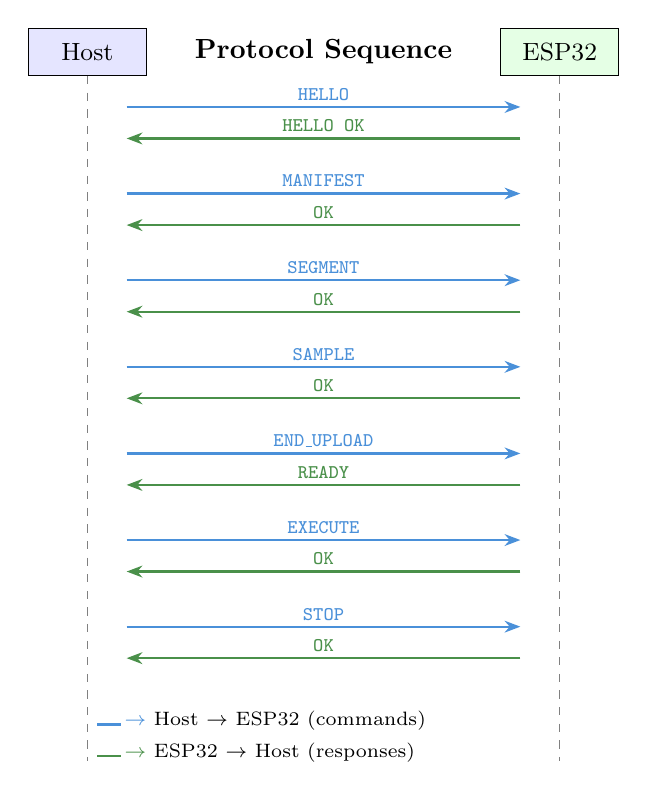
\begin{tikzpicture}[node distance=0.35cm]

\node[font=\bfseries] at (3, 0) {Protocol Sequence};

% Actors
\node[box, fill=blue!10] (host) at (0, 0) {Host};
\node[box, fill=green!10] (esp) at (6, 0) {ESP32};

% Lifelines
\draw[dashed, gray] (host) -- (0, -9);
\draw[dashed, gray] (esp) -- (6, -9);

% ── Handshake ──
\draw[toesp] (0.5, -0.7) -- node[msg, above] {HELLO} (5.5, -0.7);
\draw[tohost] (5.5, -1.1) -- node[msg, above] {HELLO OK} (0.5, -1.1);

% ── Upload ──
\draw[toesp] (0.5, -1.8) -- node[msg, above] {MANIFEST} (5.5, -1.8);
\draw[tohost] (5.5, -2.2) -- node[msg, above] {OK} (0.5, -2.2);

\draw[toesp] (0.5, -2.9) -- node[msg, above] {SEGMENT} (5.5, -2.9);
\draw[tohost] (5.5, -3.3) -- node[msg, above] {OK} (0.5, -3.3);

\draw[toesp] (0.5, -4.0) -- node[msg, above] {SAMPLE} (5.5, -4.0);
\draw[tohost] (5.5, -4.4) -- node[msg, above] {OK} (0.5, -4.4);

\draw[toesp] (0.5, -5.1) -- node[msg, above] {END\_UPLOAD} (5.5, -5.1);
\draw[tohost] (5.5, -5.5) -- node[msg, above] {READY} (0.5, -5.5);

% ── Execute ──
\draw[toesp] (0.5, -6.2) -- node[msg, above] {EXECUTE} (5.5, -6.2);
\draw[tohost] (5.5, -6.6) -- node[msg, above] {OK} (0.5, -6.6);

% ── Safety ──
\draw[toesp] (0.5, -7.3) -- node[msg, above] {STOP} (5.5, -7.3);
\draw[tohost] (5.5, -7.7) -- node[msg, above] {OK} (0.5, -7.7);

% Legend
\node[font=\scriptsize, anchor=west] at (0, -8.5) {{\color{hostblue}\rule{3mm}{1pt}\,$\to$} Host $\to$ ESP32 (commands)};
\node[font=\scriptsize, anchor=west] at (0, -8.9) {{\color{espsoft}\rule{3mm}{1pt}\,$\to$} ESP32 $\to$ Host (responses)};

\end{tikzpicture}
\end{document}
